\documentclass[conference]{IEEEtran}
\IEEEoverridecommandlockouts
\usepackage{cite}
\usepackage{amsmath,amssymb,amsfonts}
\usepackage{graphicx}
\usepackage{textcomp}
\usepackage{xcolor}
\usepackage{booktabs}
\usepackage{url}
\def\BibTeX{{\rm B\kern-.05em{\sc i\kern-.025em b}\kern-.08em
    T\kern-.1667em\lower.7ex\hbox{E}\kern-.125emX}}
% Red marker for anything that still needs a result, citation or approval number.
\newcommand{\pending}[1]{\textcolor{red}{[#1]}}
\begin{document}

\title{Patient-based Real Time Quality Control\\
\textit{A Comparison between an LSTM Autoencoder and Traditional Statistical Techniques}}

\author{\IEEEauthorblockN{1\textsuperscript{st} Zi En Tham}
\IEEEauthorblockA{
\textit{University of Technology Sydney}\\
Sydney, Australia \\
ZiEn.Tham@alumni.uts.edu.au}
}

\maketitle

\begin{abstract}
Patient-Based Real-Time Quality Control (PBRTQC) monitors the running statistics of patient results to detect analytical error between scheduled quality-control runs. Most implementations use variants of the Average of Normals (AON), such as the moving average (MA). This study asks whether an unsupervised Long Short-Term Memory (LSTM) autoencoder can improve on statistical detectors. Using 91 days of de-identified Westmead Hospital sodium and creatinine results, every test day is replayed once clean and once with a step shift of $\pm$1--20\% injected after the 300th result. All detectors (MA, EWMA, CUSUM and LSTM autoencoders) see identical streams, have their limits calibrated on clean days to the same nominal false-alarm budget without using anomaly labels, and have their parameters chosen on validation days. Performance is reported as false-alarm days, detection rate and detection delay in results. For sodium, calibrated statistical detectors flag a 5\% shift after a median of 9--11 results and a 3\% shift after 20--38, whereas an MA with $\pm3$ SD limits on raw results does not detect shifts below 10\%, which shows that baseline calibration alone can dominate any comparison with machine learning. For creatinine, all statistical detectors detect only $\approx$20\% shifts reliably (94--97\% of days, median delay about 95--110 results) because of large between-patient variability. Neither LSTM autoencoder improves on the calibrated statistical detectors, and this holds across a range of false-alarm budgets. For sodium, the better variant (with moving-average preprocessing) detects shifts of 3\% and above on every day but needs about twice the delay of MA, EWMA and CUSUM (median 18 results at 5\%, against 9--11); for creatinine both LSTMs are at or below the statistical detectors, and one exceeds its false-alarm budget on the test days. The observed false-alarm rate of the calibrated detectors on the 18 test days ranged from 0.06 to 0.28 against a nominal 0.10, and these results come from one training run per model.
\end{abstract}

\begin{IEEEkeywords}
PBRTQC, LSTM autoencoder, anomaly detection, moving average, quality control
\end{IEEEkeywords}

\section{Introduction}
Clinical laboratories depend on quality control (QC) to ensure that analysers produce accurate results. Traditionally QC samples are run at fixed intervals, so an error that starts just after a run can go unnoticed, and affect patient results, until the next one. Patient-Based Real-Time Quality Control (PBRTQC) instead monitors a statistic of consecutive patient results and raises an alarm when it drifts from the expected value for that population. Alarms can arise from calibration problems, reagent faults or sample-handling errors, and PBRTQC lets laboratories react to them as they occur rather than at the next scheduled run.

The oldest PBRTQC technique, the Average of Normals (AON) \cite{Cembrowski1984}, has many variants; this study uses the moving average (MA) as its representative statistical baseline, together with two classical change-detection charts (EWMA and CUSUM). Recurrent neural networks are widely used for sequence anomaly detection, which raises the question of whether an LSTM autoencoder offers any advantage in PBRTQC. This paper compares them under a protocol that is deliberately strict about \emph{how} detectors are compared, because we found that the comparison is easily distorted by baseline calibration and by evaluation choices (Section~\ref{sec:discussion}).

\subsection{Background}
As described by \cite{Badrick2020}, PBRTQC uses the statistical characteristics of the patient population served by a laboratory on a specific analytical platform. For AON, the average of a block of patient results should stay close to the population's expected average, and a deviation indicates a potential problem. The MA recalculates the average as each new result arrives: the oldest result of the block is dropped, so the block size sets the trade-off between speed and noise. The user chooses the block size, control limits and truncation limits (concentrations beyond which results are excluded). Depending on error size, assay precision and population distribution, several patient results may pass before an error is detected \cite{Bietenbeck2020}.

\subsection{Aims and Contributions}
The aim is to determine whether an unsupervised LSTM autoencoder detects analytical shifts faster, or at lower false-alarm cost, than calibrated statistical detectors. The contributions are:
\begin{itemize}
  \item A reproducible simulation protocol in which every detector sees identical streams, limits are calibrated to an equal nominal false-alarm budget on clean data only, and parameters are selected on validation days.
  \item Detection rate and delay in results, rather than point-wise accuracy, as the performance measures.
  \item A comparison of MA, EWMA, CUSUM and LSTM autoencoders (with and without MA preprocessing) for sodium and creatinine.
\end{itemize}
This is an exploratory, single-site study of one error type. It does not estimate cost savings or patient-outcome effects.

\section{Related Work}
Spies et al.\ \cite{Spies2023} note that most laboratory data are unlabelled, so supervised models are hard to train, and that semi-supervised and generative approaches are difficult to validate against real patient biology. Reconstruction-based LSTM models learn normal behaviour and flag sequences they reconstruct poorly; Malhotra et al.\ \cite{Malhotra2015} showed this for process monitoring without pre-specified window lengths, and Maleki et al.\ \cite{Maleki2021} applied LSTM autoencoders to unsupervised time-series anomaly detection while noting their memory and complexity costs.

Within PBRTQC itself, Duan et al.\ \cite{Duan2021} added a regression step before the statistical chart (for example an MA) to remove autocorrelation in the results and to allow further variables, and reported that regression-adjusted real-time QC (RARTQC) outperformed conventional PBRTQC. Zhou et al.\ \cite{Zhou2022} proposed a machine-learning real-time QC model built from patient data, Man et al.\ \cite{Man2023} pre-classified patients before applying real-time QC and reported gains over RARTQC, and Liang et al.\ \cite{Liang2024} extended RARTQC with a machine-learning nonlinear regression in a multi-centre study. Our study differs in three ways: the LSTM autoencoder is unsupervised and sees only one univariate result stream, with no patient variables; every detector, statistical or neural, is calibrated to the same nominal false-alarm budget on clean data and compared on identical streams; and we report detection delay and the cases in which the LSTM brings no advantage, rather than a single accuracy figure.

\section{Population and Sample Description}
The data are results from Westmead Hospital recorded between 31 December 2022 and 31 March 2023 (440,093 records across analytes, of which this study uses 64,691 sodium and 65,205 creatinine results over 91 days, a median of about 775 results per day; the first day holds only four results). The laboratory released the data to the author as de-identified quality-improvement data, without names or other direct personal details. The extract carried a pseudonymised MRN and an accession-number field, which were not used by any model.

Patients range from infants to those over 100 years old, and samples come from emergency, cancer and other wards. The results were reported laboratory results; no systematic analytical error was identified in them, and the training data are treated as in-control, which is an assumption (Section~\ref{sec:discussion}).

Figure~\ref{fig:crea_sod_distribution} shows the distributions. Sodium is approximately symmetric but more peaked than a normal distribution and has a heavier lower tail. Creatinine is strongly positively skewed. Figure~\ref{fig:crea_sod_distribution_2} shows both analytes over time.

\begin{figure}[h!]
    \centering
    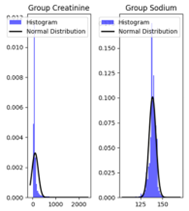
\includegraphics[width=0.3\textwidth]{resources/crea_sod_distribution.png}
    \caption{Sodium and creatinine distributions with fitted normal curves.}
    \label{fig:crea_sod_distribution}
\end{figure}

\begin{figure}[h!]
    \centering
    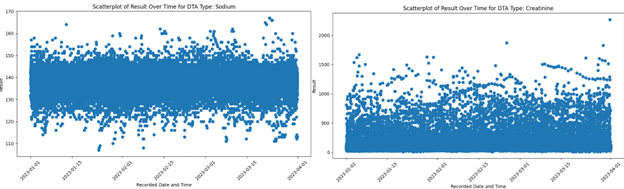
\includegraphics[width=0.5\textwidth]{resources/crea_sod_distribution_2.png}
    \caption{Sodium and creatinine results over time.}
    \label{fig:crea_sod_distribution_2}
\end{figure}

\section{Methodology}
Each day is one stream, processed independently, with no state carried across midnight. Results are first truncated (creatinine only: results above 150~\textmu mol/L are excluded, following \cite{Lukic2019}; sodium is not truncated) and then standardised using the mean $\mu$ and standard deviation $\sigma$ of the training days after truncation (sodium $138.4\pm4.0$~mmol/L; creatinine $73.4\pm25.4$~\textmu mol/L). The same preprocessing is used for every detector. Each detector produces a score $s_t$ using only results up to $t$, and raises an alarm when $s_t$ exceeds a limit.

\subsection{Statistical Detectors}
With standardised results $z_i$, the moving average over block size $n$ is
\[
MA_t = \frac{1}{n}\sum_{i=t-n+1}^{t} z_i, \qquad s_t = |MA_t|,
\]
with no score until $n$ results are available \cite{Bietenbeck2020}. The EWMA is $e_t=\lambda z_t+(1-\lambda)e_{t-1}$ with $s_t=|e_t|$. The two-sided CUSUM keeps $S^{+}_t=\max(0,S^{+}_{t-1}+z_t-k)$ and $S^{-}_t=\max(0,S^{-}_{t-1}-z_t-k)$ with $s_t=\max(S^{+}_t,S^{-}_t)$.

\subsection{Limit Calibration}
\label{sec:calibration}
The limit of each detector is the $q$-quantile ($q=0.9$) of the \emph{daily maxima} of its score over clean calibration days:
\[
L=Q_q\Big(\big\{\max_t s^{(d)}_t\big\}_{d\in\mathcal{D}_{cal}}\Big).
\]
This aims at roughly one false-alarm day in ten for every detector, so detectors are compared at an equal nominal false-alarm budget, and it uses no anomaly labels. The statistical detectors have no trained parameters, so training and validation days form $\mathcal{D}_{cal}$; the LSTM limits use validation days only. As a reference, an \emph{uncalibrated} MA ($n=50$) with the fixed limits $\pm3\sigma$ of the raw results (the usual Shewhart setting, applied here to the block average) is also evaluated. Because the standard deviation of a 50-point mean is about $\sigma/\sqrt{50}$, such limits are roughly seven times wider than the variation of the statistic itself.

\subsection{LSTM Autoencoder}
A stacked LSTM autoencoder (encoder 64--32--16 units, repeat vector, decoder 16--32 units, time-distributed dense output, 20\% dropout; Fig.~\ref{fig:model_summary}) is trained only on in-control training days to reconstruct windows of $T=70$ consecutive results. Training windows never cross a day boundary. Two variants are used: LSTM-AE on the standardised results, and LSTM-AE-MA, whose input is first smoothed by a 50-result moving average. The model is trained with Adam and mean squared error, with early stopping (patience 5) on the held-out validation days, and its inputs are divided by a constant training standard deviation.

At test time the score $s_t$ is the reconstruction mean squared error of the window of the last $T$ (smoothed) results ending at $t$, so an alarm can be raised after every result and its delay is measured exactly like the statistical detectors. Its limit is calibrated with the same procedure as above.

\begin{figure}[h!]
    \centering
    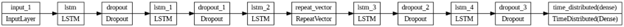
\includegraphics[width=0.5\textwidth]{resources/model_summary.png}
    \caption{LSTM autoencoder architecture.}
    \label{fig:model_summary}
\end{figure}

\section{Experimental Design}
\subsection{Data Split}
The 91 days are split chronologically by whole days into 55 training, 18 validation and 18 test days. Random shuffling is not used, because it destroys the time order.

\subsection{Shift Simulation}
A test day with at least 400 results is replayed twice. In the clean replay, any alarm is a false alarm. In the shifted replay, every result from the 301st onwards is multiplied by $1+b$, with $b\in\{\pm1,\pm2,\pm3,\pm5,\pm10,\pm20\}\%$; the shift persists to the end of the day. All 18 test days qualified, so each detector was run on 18 clean and $12\times18$ shifted streams.

The shift is applied to the raw results before truncation and standardisation, as an analyser bias would be. It is therefore a proportional bias and not a pure location shift. It moves the mean of the standardised stream by about $b\mu/\sigma$ (for sodium $34.7\,b$ SD, so $+1.7$ SD at 5\%) and also scales its spread by about $1+b$ (for sodium the SD of the monitored results is 1.20 times its unshifted value at $+20\%$ and 0.80 times at $-20\%$). For creatinine the truncation limit interacts with the shift: a $+20\%$ shift pushes 4.3\% of the results over 150~\textmu mol/L out of the monitored stream and a $-20\%$ shift brings 3.1\% more results into it. The effective mean shifts are therefore $+0.44$ and $-0.49$ SD against a nominal $\pm0.58$ (at 5\%: $+0.11$ and $-0.12$ SD against $\pm0.14$), and positive and negative shifts are not mirror images. Constant (additive) offsets were not simulated.

\subsection{Parameter Selection}
Detector parameters (MA $n\in\{20,50,100\}$; EWMA $\lambda\in\{0.02,0.05,0.1,0.2\}$; CUSUM $k\in\{0.25,0.5\}$) are chosen on the validation days as the value with the lowest mean detection delay at $\pm5\%$ shifts, counting an undetected shift as the full remaining day. The test days are not used for any choice. For creatinine, a 5\% shift is near the detection floor (at most 14\% of test days are detected), so the choice is made on very little signal and the creatinine parameters are the least reliable.

\subsection{Evaluation Metrics}
\begin{itemize}
  \item \textbf{False-alarm day rate}: fraction of clean test days with at least one alarm.
  \item \textbf{Detection rate}: fraction of shifted days with an alarm at or after the shift onset.
  \item \textbf{Detection delay}: number of results between the onset and the first alarm, reported as the median over days (``--'' when fewer than half the days are detected). Delay is counted in original results, so truncated results still count as time passing. It equals the number of results reported with an erroneous value before the alarm; repeat results from one patient were not de-duplicated, so it overcounts unique patients.
  \item \textbf{Detection delay in minutes}: the same delay converted to minutes of recorded time using the timestamp of the result at the shift onset and of the alarming result. It is a supplement, because the laboratory records results in bursts.
\end{itemize}
Point-wise accuracy is not reported: with roughly 60\% of points shifted it mostly reflects prevalence, and consecutive flags from one excursion are not independent alarms. Positive and negative shifts are scored separately, and Table~\ref{experiment_result} averages the two.

\subsection{Operating Curves}
To check that the conclusions do not depend on a single false-alarm budget, every calibrated detector is also evaluated at $q\in\{0.5,0.7,0.8,0.9,0.95,0.98\}$. The scores are computed once and only the limit changes. The fixed-limit MA is excluded because it has no budget to vary.

\section{Results}
Table~\ref{experiment_result} gives the results, averaging the positive and negative shifts of each magnitude. The selected parameters were MA $n=20$, EWMA $\lambda=0.1$ and CUSUM $k=0.5$ for sodium, and MA $n=100$, EWMA $\lambda=0.02$ and CUSUM $k=0.25$ for creatinine.

\begin{table*}[!t]
\centering
\renewcommand{\arraystretch}{1.15}
\setlength{\tabcolsep}{5pt}
\caption{Detection rate (median delay in results) on the 18 test days. FA is the false-alarm day rate on the clean replay. Values average the $+$ and $-$ shift of each magnitude (separate values are in the results files); ``--'' means fewer than half of the days were detected.}
\label{experiment_result}
\begin{tabular}{llc cccccc}
\toprule
\textbf{Analyte} & \textbf{Detector} & \textbf{FA} & \textbf{1\%} & \textbf{2\%} & \textbf{3\%} & \textbf{5\%} & \textbf{10\%} & \textbf{20\%} \\
\midrule
Sodium & MA ($n{=}50$), $\pm3$ SD fixed limits & 0.00 & 0.00 (--) & 0.00 (--) & 0.00 (--) & 0.00 (--) & 1.00 (43) & 1.00 (21) \\
 & MA ($n{=}20$) & 0.11 & 0.39 (--) & 0.97 (88) & 1.00 (20) & 1.00 (11) & 1.00 (5) & 1.00 (2) \\
 & EWMA ($\lambda{=}0.1$) & 0.11 & 0.39 (--) & 0.89 (142) & 1.00 (38) & 1.00 (9) & 1.00 (3) & 1.00 (1) \\
 & CUSUM ($k{=}0.5$) & 0.06 & 0.47 (--) & 1.00 (64) & 1.00 (24) & 1.00 (10) & 1.00 (4) & 1.00 (2) \\
 & LSTM-AE & 0.11 & 0.08 (--) & 0.25 (--) & 0.47 (--) & 0.97 (95) & 1.00 (12) & 1.00 (2) \\
 & LSTM-AE-MA & 0.11 & 0.36 (--) & 1.00 (78) & 1.00 (37) & 1.00 (18) & 1.00 (8) & 1.00 (3) \\
\midrule
Creatinine & MA ($n{=}50$), $\pm3$ SD fixed limits & 0.00 & 0.00 (--) & 0.00 (--) & 0.00 (--) & 0.00 (--) & 0.00 (--) & 0.00 (--) \\
 & MA ($n{=}100$) & 0.11 & 0.03 (--) & 0.03 (--) & 0.06 (--) & 0.14 (--) & 0.47 (--) & 0.94 (95) \\
 & EWMA ($\lambda{=}0.02$) & 0.06 & 0.00 (--) & 0.00 (--) & 0.00 (--) & 0.08 (--) & 0.42 (--) & 0.94 (110) \\
 & CUSUM ($k{=}0.25$) & 0.06 & 0.00 (--) & 0.03 (--) & 0.03 (--) & 0.11 (--) & 0.44 (--) & 0.97 (95) \\
 & LSTM-AE & 0.06 & 0.00 (--) & 0.03 (--) & 0.00 (--) & 0.03 (--) & 0.03 (--) & 0.17 (--) \\
 & LSTM-AE-MA & 0.28 & 0.08 (--) & 0.11 (--) & 0.11 (--) & 0.11 (--) & 0.28 (--) & 0.89 (140) \\
\bottomrule
\end{tabular}
\end{table*}

\textbf{Sodium.} With calibrated limits, MA, EWMA and CUSUM detect every 3\% shift (median delay 20--38 results) and every 5\% shift (9--11 results), and detect a 20\% shift almost immediately (1--2 results). A 1\% shift (about 1.4~mmol/L) is detected on fewer than half of the days (39--47\%, compared with a false-alarm day rate of 6--11\%). The uncalibrated MA with $\pm3$ SD limits on raw results detects nothing below 10\%, and needs a median of 43 results at 10\% where the calibrated detectors need 3--5.

\textbf{Creatinine.} Detection is much weaker. At 10\% only 42--47\% of days are flagged by the calibrated detectors, at 5\% no more than 14\%, and only a 20\% shift is detected reliably (94--97\% of days, median delay 95--110 results). The uncalibrated limits detect nothing at any magnitude.

\textbf{False alarms.} The calibration targets about 10\% of clean days. The observed rate on the test days was 6--11\% (one or two of 18 days) for every detector except LSTM-AE-MA on creatinine, which alarmed on 28\% of clean days (5 of 18), well above its budget. Its limit was calibrated on only 18 validation days, so its detection figures for creatinine are not at an equal false-alarm rate and flatter it.

\textbf{LSTM.} On sodium, LSTM-AE-MA is the better variant. It detects every shift of 2\% and above, and it is the only detector besides CUSUM to flag every 2\% shift (median 78 results, against 64 for CUSUM and 88--142 for MA and EWMA at a rate of 0.89--0.97). At 3\% it is comparable (median 37 results, against 20--38 for the statistical detectors), but from 5\% upward it is about twice as slow: 18 results at 5\% (9--11), 8 at 10\% (3--5) and 3 at 20\% (1--2). At 1\% it detects 36\% of days, no better than the statistical detectors (39--47\%). LSTM-AE without MA preprocessing is clearly worse: 47\% at 3\% and a median of 95 results at 5\%. On creatinine, LSTM-AE detects only 17\% of days even at 20\%, and LSTM-AE-MA detects 89\% at 20\% (median 140 results) against 94--97\% (95--110) for the statistical detectors, at the higher false-alarm rate noted above.

\textbf{Positive and negative shifts.} Averaging the two signs hides little for shifts of 3\% and above. No detector's detection rate differs by 0.2 or more between the signs for sodium at those sizes, and the statistical detectors differ by less than 0.2 on creatinine at every size (at most 0.11 at 20\%). Small sodium shifts are the exception: a 1\% shift is found more often when negative (MA 56\% against 22\% of days, EWMA 61\% against 17\%, CUSUM 67\% against 28\%), and the EWMA needs a median of 216 results for a $+2\%$ shift against 67 for $-2\%$. The mean of the test days lies within 0.01 SD of the training mean, so a level difference between the periods does not explain this; the heavier lower tail of sodium might, but we did not test it. With 18 days, a gap of 0.2--0.4 is 4--8 days. The LSTM variants are more asymmetric on creatinine at 20\% (LSTM-AE 28\% against 6\%, LSTM-AE-MA 78\% against 100\%).

\textbf{Delay in minutes.} Results are recorded in bursts (about 0.5 per minute averaged over the day), and the 301st result is recorded at a median of 10:17. Delays in minutes are therefore short and uneven. For sodium the calibrated statistical detectors flag a 5\% shift after a median of about one minute of recorded time (1.0--1.2), a 3\% shift after 10--24 minutes and a 2\% shift after 46--132 minutes; shifts of 10\% and above are flagged within a minute. For creatinine a 20\% shift takes 72--86 minutes. Because minutes depend on how results are batched, the number of results reported with an erroneous value is the more robust measure. LSTM-AE-MA needs about 7 minutes for a 5\% sodium shift (against about one for the statistical detectors), 22 minutes for 3\% (10--24) and 66 for 2\% (46--132), and 109 minutes for a 20\% creatinine shift (72--86); LSTM-AE needs about 83 minutes for a 5\% sodium shift.

\textbf{Operating curves.} Table~\ref{tab:sweep} repeats the comparison at four false-alarm budgets. Sodium is insensitive to the budget: all three statistical detectors detect every 3\% and 5\% shift at every budget from $q=0.5$ to $0.95$, and only the delay changes (15--18 results at $q=0.5$ against 28--50 at $q=0.95$ for a 3\% shift). The observed test false-alarm rate tracks the budget for sodium (0.44--0.50 at $q=0.5$). Creatinine is different. Detecting a 10\% shift on 86--92\% of days requires accepting an alarm on 67--83\% of clean days ($q=0.5$), and at the 10\%-of-days budget only 42--47\% are detected. A 20\% shift is found on 94--100\% of days at every budget in the table, so the budget buys speed there: a median of 41--62 results at $q=0.5$ against 95--110 at $q=0.9$. For creatinine the observed false-alarm rate exceeds the budget (0.67--0.83 at $q=0.5$), which suggests that the calibration days are not fully representative of the test days.

The observed false-alarm rate of the LSTM variants follows the budget less closely. On sodium, LSTM-AE-MA is below it at low $q$ (0.33 at $q=0.5$) and cannot fall below one day in 18 at high $q$ (0.06); on creatinine it is above it throughout (0.61 at $q=0.5$, 0.11 at $q=0.98$). Comparing at similar observed false-alarm rates, at 35 of the 36 sodium operating points of LSTM-AE-MA (six budgets, six shift sizes) a statistical detector has an equal or lower false-alarm rate, an equal or higher detection rate and an equal or shorter delay, and the same holds at all 36 points of LSTM-AE. The exception is a 1\% shift at $q=0.7$, where LSTM-AE-MA detects 61\% of days after a median of 429 results. At a false-alarm rate of 0.06, LSTM-AE-MA detects every 2\% sodium shift (median 88 results), more reliably than MA (83\% of days) and EWMA (72\%) and nearly as fast as CUSUM (72 results), but it is slower than CUSUM at every size from 3\% to 20\% (for example 22 against 10--13 results at 5\%). On creatinine, a statistical detector does not dominate LSTM-AE-MA at 17 of the 36 points, but all of these are low-detection points (at most 47\% of days, no median delay) at false-alarm rates that fall between the statistical operating points. At a similar rate of 0.11, LSTM-AE-MA detects 19\% of 10\% shifts and 86\% of 20\% shifts (median about 160 results), against 42--47\% and 94--97\% (95--110) for the statistical detectors, and LSTM-AE detects 3\% and 17\% at a rate of 0.06.

\textbf{Uncertainty.} All rates come from 18 test days, so they are coarse. The 95\% Wilson intervals are about 82--100\% for 18 of 18 days detected, 74--99\% for 17 of 18, 67--97\% for 16 of 18, 34--75\% for 10 of 18 and 12--51\% for 5 of 18; a false-alarm rate of 1 of 18 days is 1--26\%, 2 of 18 is 3--33\% and 5 of 18 is 12--51\%. Table entries average the two signs of the same 18 days, which does not remove this uncertainty. Differences in detection or false-alarm rate below about 0.2 should therefore not be read as real, and delays, which are medians over the same days, are similarly imprecise. The conclusions that rest on large gaps are the uncalibrated MA missing 3--5\% sodium shifts, creatinine being much harder than sodium, and LSTM-AE being worse than the other detectors; statements such as ``about twice as slow'' for LSTM-AE-MA are suggestive only. The design is paired (the same days and both signs for every detector), so a paired comparison, for example a McNemar-type test on per-day detection or a bootstrap over days for the delay medians, would be appropriate; it was not performed because the per-day outcomes were not stored.

\begin{table*}[!t]
\centering
\renewcommand{\arraystretch}{1.15}
\setlength{\tabcolsep}{5pt}
\caption{Operating curves: false-alarm day rate / detection rate (median delay in results) at four false-alarm budgets $q$. Values average the $+$ and $-$ shift; ``--'' means fewer than half of the days were detected.}
\label{tab:sweep}
\begin{tabular}{lll cccc}
\toprule
\textbf{Analyte} & \textbf{Shift} & \textbf{Detector} & $q{=}0.5$ & $q{=}0.8$ & $q{=}0.9$ & $q{=}0.95$ \\
\midrule
Sodium & 3\% & MA ($n{=}20$) & 0.44 / 1.00 (16) & 0.11 / 1.00 (18) & 0.11 / 1.00 (20) & 0.06 / 1.00 (35) \\
 & 3\% & EWMA ($\lambda{=}0.1$) & 0.50 / 1.00 (18) & 0.33 / 1.00 (22) & 0.11 / 1.00 (38) & 0.06 / 1.00 (50) \\
 & 3\% & CUSUM ($k{=}0.5$) & 0.44 / 1.00 (15) & 0.28 / 1.00 (18) & 0.06 / 1.00 (24) & 0.06 / 1.00 (28) \\
 & 3\% & LSTM-AE & 0.56 / 0.92 (168) & 0.44 / 0.72 (314) & 0.11 / 0.47 (--) & 0.06 / 0.33 (--) \\
 & 3\% & LSTM-AE-MA & 0.33 / 1.00 (31) & 0.17 / 1.00 (36) & 0.11 / 1.00 (37) & 0.06 / 1.00 (41) \\
\cmidrule(lr){2-7}
 & 5\% & MA ($n{=}20$) & 0.44 / 1.00 (9) & 0.11 / 1.00 (10) & 0.11 / 1.00 (11) & 0.06 / 1.00 (13) \\
 & 5\% & EWMA ($\lambda{=}0.1$) & 0.50 / 1.00 (6) & 0.33 / 1.00 (8) & 0.11 / 1.00 (9) & 0.06 / 1.00 (12) \\
 & 5\% & CUSUM ($k{=}0.5$) & 0.44 / 1.00 (6) & 0.28 / 1.00 (8) & 0.06 / 1.00 (10) & 0.06 / 1.00 (12) \\
 & 5\% & LSTM-AE & 0.56 / 1.00 (37) & 0.44 / 1.00 (50) & 0.11 / 0.97 (95) & 0.06 / 0.94 (117) \\
 & 5\% & LSTM-AE-MA & 0.33 / 1.00 (15) & 0.17 / 1.00 (17) & 0.11 / 1.00 (18) & 0.06 / 1.00 (22) \\
\midrule
Creatinine & 10\% & MA ($n{=}100$) & 0.83 / 0.92 (134) & 0.33 / 0.69 (297) & 0.11 / 0.47 (--) & 0.00 / 0.22 (--) \\
 & 10\% & EWMA ($\lambda{=}0.02$) & 0.67 / 0.89 (126) & 0.39 / 0.83 (202) & 0.06 / 0.42 (--) & 0.00 / 0.22 (--) \\
 & 10\% & CUSUM ($k{=}0.25$) & 0.67 / 0.86 (117) & 0.06 / 0.58 (--) & 0.06 / 0.44 (--) & 0.00 / 0.28 (--) \\
 & 10\% & LSTM-AE & 0.33 / 0.08 (--) & 0.06 / 0.03 (--) & 0.06 / 0.03 (--) & 0.00 / 0.00 (--) \\
 & 10\% & LSTM-AE-MA & 0.61 / 0.61 (--) & 0.39 / 0.33 (--) & 0.28 / 0.28 (--) & 0.22 / 0.22 (--) \\
\cmidrule(lr){2-7}
 & 20\% & MA ($n{=}100$) & 0.83 / 1.00 (62) & 0.33 / 0.97 (90) & 0.11 / 0.94 (95) & 0.00 / 0.94 (117) \\
 & 20\% & EWMA ($\lambda{=}0.02$) & 0.67 / 1.00 (48) & 0.39 / 0.97 (62) & 0.06 / 0.94 (110) & 0.00 / 0.94 (133) \\
 & 20\% & CUSUM ($k{=}0.25$) & 0.67 / 0.97 (41) & 0.06 / 0.97 (77) & 0.06 / 0.97 (95) & 0.00 / 0.94 (130) \\
 & 20\% & LSTM-AE & 0.33 / 0.39 (--) & 0.06 / 0.19 (--) & 0.06 / 0.17 (--) & 0.00 / 0.08 (--) \\
 & 20\% & LSTM-AE-MA & 0.61 / 0.97 (101) & 0.39 / 0.89 (127) & 0.28 / 0.89 (140) & 0.22 / 0.86 (159) \\
\bottomrule
\end{tabular}
\end{table*}

\section{Discussion}
\label{sec:discussion}

\subsection{Baseline Calibration Dominates the Comparison}
The uncalibrated MA fails below 10\% only because its limits, set at $\pm3\sigma$ of raw results, are far wider than the spread of a block average. Re-scaled to the false-alarm budget, the same statistic, and EWMA and CUSUM, detect a 3\% sodium shift within a few tens of results. Any claim that machine learning outperforms ``the moving average'' therefore needs the MA limits to be calibrated, and ideally compared with EWMA/CUSUM, at the same false-alarm rate. Against calibrated baselines, the LSTM autoencoders gave no advantage over the best statistical detector (CUSUM) at any false-alarm budget we tested; the only gain was over MA and EWMA for 2\% sodium shifts at low false-alarm rates.

\subsection{What a 5\% Sodium Shift Means}
A 5\% sodium shift is about 7~mmol/L, which is not subtle clinically. The RCPA analytical performance specifications for serum sodium (minimal total-error basis) are $\pm3$~mmol/L up to 150~mmol/L and $\pm2\%$ above \cite{RCPA}, and total error includes imprecision as well as bias. At the training mean of 138~mmol/L a 3\% shift is 4.1~mmol/L and a 2\% shift is 2.8~mmol/L, so shifts of 2--3\% already consume the whole allowance, and a 5\% shift is more than twice it. The 1\% shift (1.4~mmol/L) is the only simulated magnitude within the allowance, and it is also the only one the detectors could not reliably find. Failing to detect a 5\% shift is therefore a failure, not a harmless limit of a method. Detection depends on the shift relative to the variation of the monitored statistic (many consecutive results), not on whether individual results leave the reference interval.

\subsection{Why the LSTM Does Not Help}
We did not test the mechanism, but the pattern is consistent with the LSTM acting mainly as a level detector. A step change in the mean is the only kind of anomaly in this simulation, and the reconstruction error of a window grows with how far the level has moved from the training range. The score is only available once a window of 70 smoothed results is full, and each smoothed value averages 50 results, so the detector looks over about 120 results. That makes it slower than an MA, EWMA or CUSUM that responds directly to the latest results. MA preprocessing helps because it removes noise the autoencoder cannot predict anyway, and without it the LSTM fails on small shifts. The creatinine false-alarm overshoot, which also affects the statistical detectors at low $q$, suggests that the calibration days are not fully representative of the test days; an LSTM whose limit comes from only the 18 validation days that also select its training epoch is the most exposed. An LSTM would be expected to help only for anomaly types that carry temporal structure, such as drift, cyclical patterns or changes in variability, which were not simulated here.

\subsection{Why Creatinine Is Hard}
After truncation the creatinine standard deviation is 25.4~\textmu mol/L, so a 5\% shift of the mean (about 3.7~\textmu mol/L) is only about 0.15 SD. A mean-shift detector needs roughly $(3/0.15)^2\approx 400$ results to separate it from noise, which is more than the 100 to roughly 600 post-onset results available per day in this design. Larger shifts (20\%) are detected within about 100 results. Population mixing across wards and analysers likely adds to this and was not modelled. Wider truncation limits, transformation, and stratified or continuous (multi-day) monitoring are the obvious next steps.

\subsection{Evaluation Pitfalls}
Three choices can bias PBRTQC simulations. (i) \emph{Rolling statistics carried across day boundaries} let a biased evening contaminate the next morning's clean results, which then appear as false positives whose rate varies with the bias size. Each day is processed independently here. (ii) \emph{Point-wise accuracy} depends on the share of shifted points (about 60\% here), so it can reach 40\% for a detector that never alarms; false-alarm days and detection delay are what a laboratory experiences. (iii) \emph{Overlapping windows} counted as separate points repeat the same result many times and, if the prediction and label sets are not built identically, misalign them. Delay measured per alarm avoids both. We met (i) and (iii) in a preliminary version of this work whose pipeline was superseded and is not reported here, so they are listed as hazards to check, not as findings of this study.

\subsection{Limitations}
The study uses one hospital, three months of data, 18 test days, one error type (a multiplicative step shift starting at result 300 and persisting for the rest of the day), and processes each day separately, so slow drift, constant offsets, imprecision changes and continuous monitoring are not covered. Training data are assumed in control, though analytical shifts, lot changes and calibrations could be present. Repeat results from one patient were not de-duplicated, so successive results are not fully independent, and the same patients may appear in training and test days. Quantile-based limits assume the clean distribution is stationary, and with 18 test days the false-alarm rates are coarse. Each LSTM was trained once (seed 0), so run-to-run variability and confidence intervals are not reported, and differences of a few results between the better LSTM and the statistical detectors should not be over-read. Parameters tuned here may not transfer to other laboratories \cite{Bietenbeck2020}. Each LSTM trained for roughly 10--20 minutes on a T4 GPU (about 25 s per epoch, with early stopping), whereas the statistical detectors run instantly. The shift always starts at the 301st result of the day (a median of 10:17, a period of high throughput), and delay depends on throughput at the onset, so shifts that start at other times of day were not simulated. The false-alarm budget of about one day in ten is generous and is a day-level measure; average run length was not estimated, although the operating curves show the trade-off down to $q=0.98$. The statistical detectors were calibrated on 73 days but the LSTM limits on only 18, and those 18 days also select the LSTM's training epoch, so the comparison is not balanced. With 18 days the 0.9-quantile is interpolated between the second and third largest daily maxima, so the LSTM limits rest on one or two effective points, and the LSTM false-alarm rates (0.33 at $q=0.5$ for sodium, 0.61 for creatinine, 0.28 at $q=0.9$ for creatinine) have wide, unquantified uncertainty. The LSTM comparison is therefore disadvantaged in calibration, and its false-alarm figures should be read as rough. The LSTM settings (window length, MA window, architecture) come from earlier exploratory work and were not tuned in this protocol, whereas the statistical parameters were selected on validation days.

\subsection{Future Work}
Next steps are: simulating drift, constant offsets, variance changes and cyclical errors, where a recurrent model might help; randomising the shift onset across the day; training several seeds per LSTM with calibration days separate from the early-stopping days; adding a regression-adjusted baseline that uses patient variables such as ward, age and time of day; estimating average run length; storing per-day outcomes for paired tests and bootstrap intervals; and validating on further sites and periods.

\section*{Reproducibility and Data Availability}
The results in this paper cannot be independently reproduced. The patient results were released to the author by the laboratory as quality-improvement data and are not publicly available, so a reader cannot regenerate Tables~\ref{experiment_result} and~\ref{tab:sweep} without the laboratory's permission. The LSTM results come from a single training run on a GPU, which is not bitwise repeatable, so even with the same data a retrained model may differ slightly. The methods, settings and splits are described above so that the study can be repeated on other laboratories' own results, which would test whether the findings hold elsewhere.

\section*{Conclusion}
Using an evaluation in which every detector sees identical streams, limits are calibrated to the same nominal false-alarm budget on clean data, and parameters are chosen on validation days, calibrated statistical detectors detect 3--5\% sodium shifts within about 10--40 results, while an MA with limits set from the raw-result spread misses everything below 10\%. For creatinine only 20\% shifts are detected reliably by any statistical detector, owing to large between-patient variation. The unsupervised LSTM autoencoders did not improve on these detectors: the better variant (with MA preprocessing) was comparable at 1--3\% sodium shifts and about twice as slow at 5--20\%, and both were weaker on creatinine. Across six false-alarm budgets a statistical detector matched or beat LSTM-AE-MA at 35 of 36 sodium operating points, with a small gain only over MA and EWMA for 2\% shifts at low false-alarm rates. A step shift in the mean, the only anomaly simulated, gives a recurrent model nothing to exploit beyond the level. Whether LSTMs help for drift, variance change or cyclical error remains untested. The study also shows that baseline calibration and evaluation design can matter as much as the choice of model, so claims of machine-learning superiority in PBRTQC should be tested against calibrated baselines at equal false-alarm rates.

\bibliographystyle{IEEEtran}
\bibliography{reference}
\end{document}
